\section{Destination Data Management}\label{sec:DestinationDataManagement}
\subsection{Problem Statement}
To facilitate destination queries, it is necessary to store relevant metadata about each place in a well-organized and accessible manner. For instance, for a room, details such as its building name, room code, purpose, and physical location are essential elements that enable users to narrow down their search quickly and accurately. This metadata is the foundational layer for advanced search functionalities, ensuring that even vague or partial user input can be matched to the correct destination. To manage and retrieve this wealth of information efficiently, building a robust database tailored to the specific needs of destination queries is essential.

\subsection{Solutions}
Large Language Models (LLMs) have revolutionized how natural language is processed by leveraging deep learning architectures trained on vast text corpora. These models excel at understanding context, generating coherent responses, and capturing subtle nuances in language, which make them ideal for interpreting and matching user queries to relevant destination metadata. By integrating LLMs, the solutions can efficiently bridge the gap between unstructured input and structured data, enabling more flexible, accurate, and context-aware search functionalities.

Leveraging the ability of LLMs to process natural language, we have explored three approaches to address this challenge.

\subsubsection{Solution 1: Description Matching}\label{description-matching}
As the most straightforward approach, we store the entire description of each place in the database. When there is a need to query a place, we feed all the place descriptions to the LLMs and ask them to find the best fit. This method ensures that the context is fully preserved, and the correct place is likely to be found most of the time. However, a downside is that it demands substantial storage space. As the number of places increases, storing and searching through large volumes of data becomes expensive and computationally intensive.

\subsubsection{Solution 2: Keyword Matching}
To reduce storage space, for each place we extract and store its most relevant keywords using the LLMs. We apply a reverse index technique, i.e., an edge linking that keyword to the corresponding place is stored for each keyword. Since some keywords are pretty similar (i.e., different keywords describing the same attribute), for example, there might be two rooms with the keywords \texttt{toilet} and \texttt{restroom}, respectively, and the user asks for the nearest \texttt{lavatory}. In this case, both rooms satisfy the query. Therefore, we try to group them under the same keyword. For example, when considering those keywords, \textbf{restroom} can be used uniformly.

To check if the keywords are similar enough to be grouped together, we use vector embeddings. Vector embeddings map words or phrases into a high-dimensional space, where the distance between vectors represents the semantic similarity between their corresponding keywords. We convert each keyword into its vector representation using the LLMs. We then compute the cosine similarity between these vectors to measure how close or related they are. If the similarity score between two keywords exceeds a predefined threshold, we infer that they convey the same or similar meaning, and therefore, we group them under a unified keyword. A sample structure is illustrated in Figure~\ref{fig:data-management-1}.

\begin{figure}[ht]
  \centering
  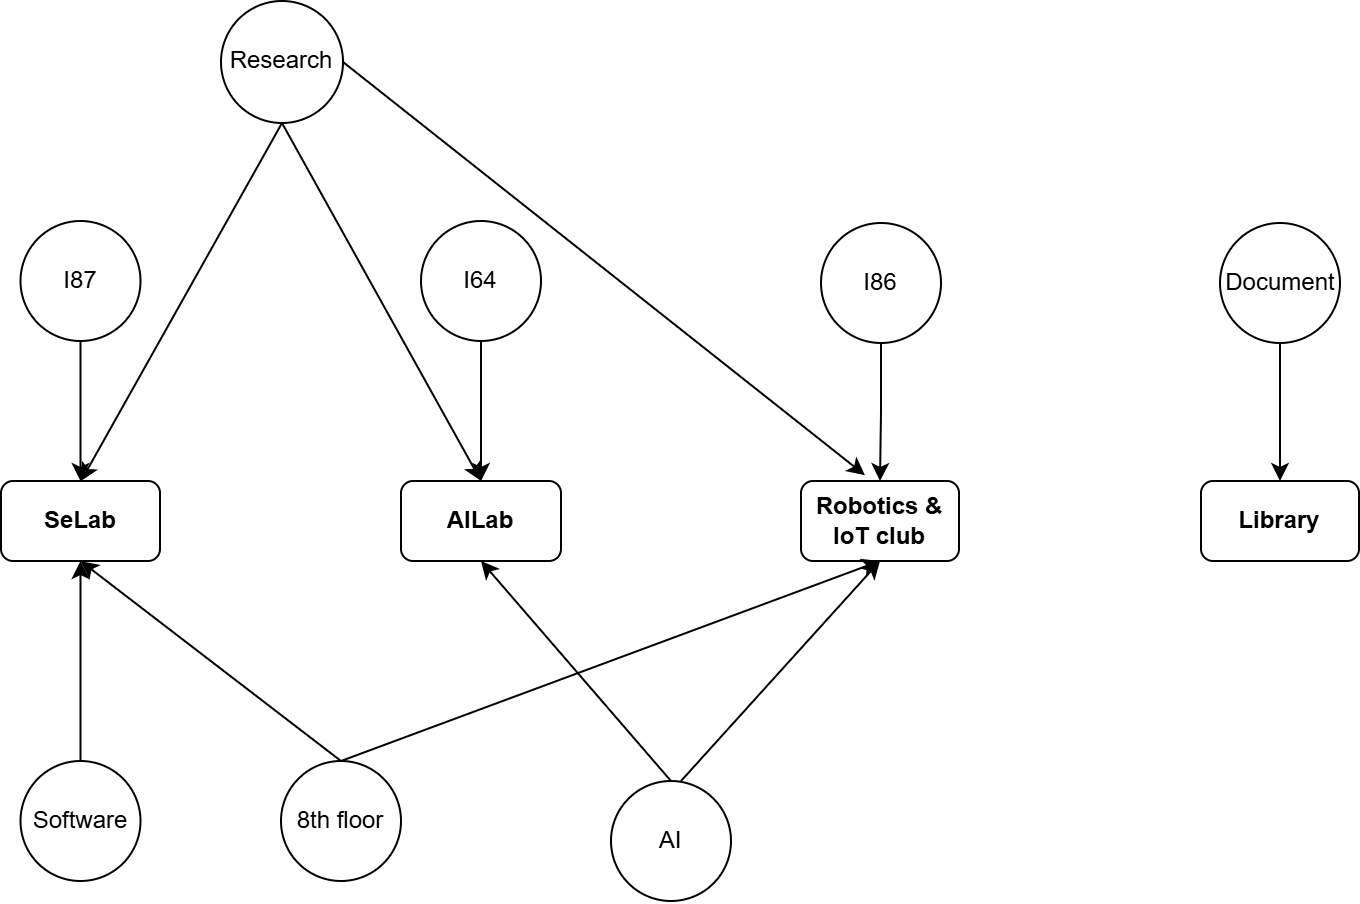
\includegraphics[scale=0.3]{content/resources/images/chap-problems-solutions/data-management-1.png}
  \caption{Keywords graph for four different rooms (square). The keywords are described as nodes (circles).}
  \label{fig:data-management-1}
\end{figure}

When processing a user query for a room, our system first extracts the pertinent keywords. The matching process then involves identifying the room that best corresponds to these keywords. The best match is the room with the highest number of keyword references or ideally contains all the keywords extracted from the query. For instance, if the user provides the following query:

\begin{lstlisting}[style=cSharp]
Please find me the laboratory of software on the 8th level.
\end{lstlisting}

The keywords extracted by the LLM are \texttt{laboratory}, \texttt{software}, and \texttt{8th level}. Using vector embeddings, these can be matched with the defined keys in the database, which are \texttt{research}, \texttt{software}, and \texttt{8th floor}, respectively. Then, the \texttt{SeLab}, \texttt{AILab}, and \texttt{Robotics \& IoT club} are referenced three times, twice, and once, respectively, as shown in Figure~\ref{fig:data-management-2}. Therefore, the \texttt{SeLab} is the desired destination.

\begin{figure}[ht]
  \centering
  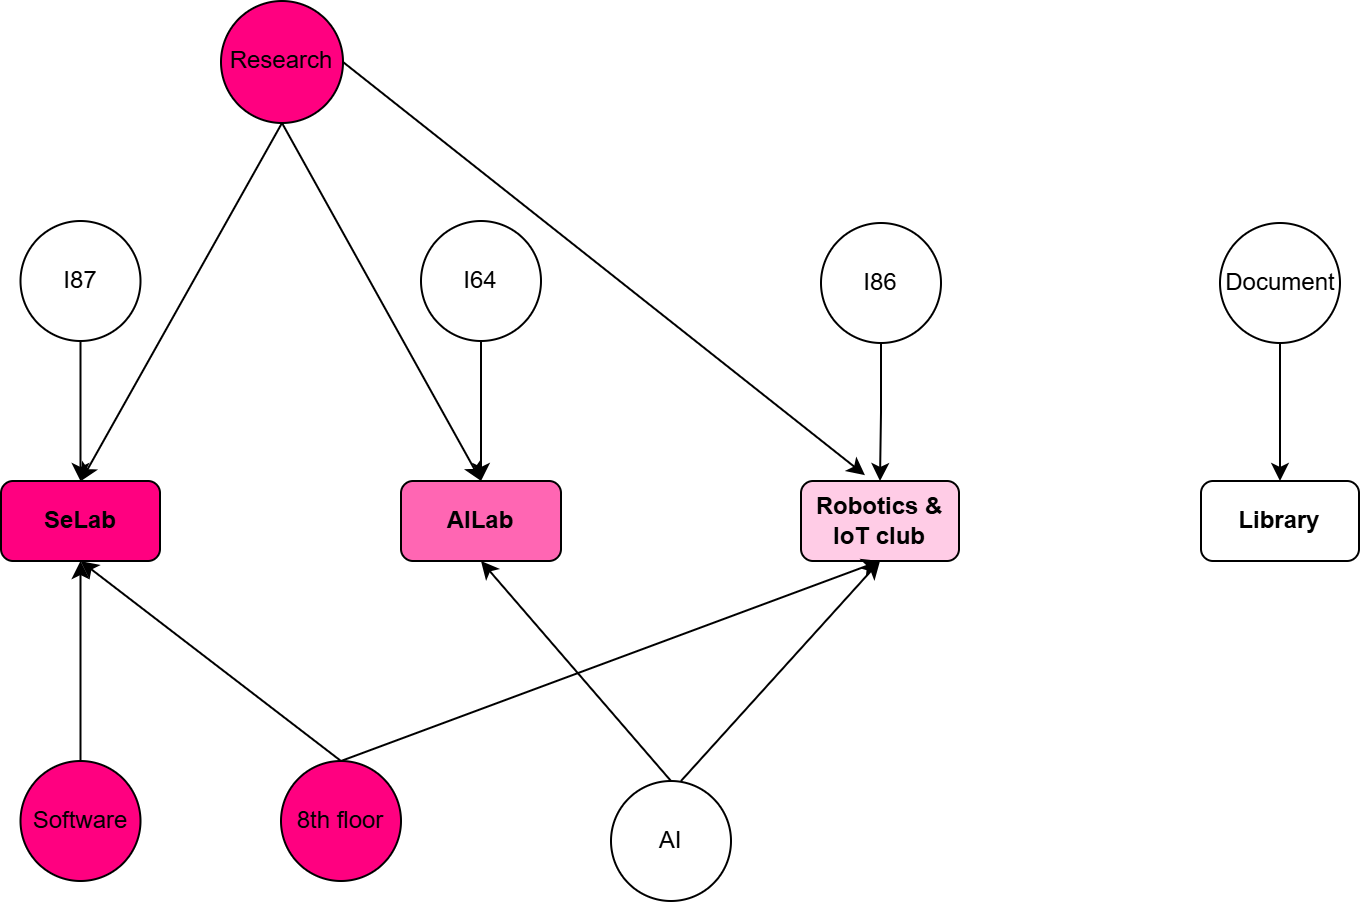
\includegraphics[scale=0.3]{content/resources/images/chap-problems-solutions/data-management-2.png}
  \caption{Reference to rooms with keywords.}
  \label{fig:data-management-2}
\end{figure}

While this approach is efficient in terms of storage and retrieval, it does have certain limitations. A notable downside is that relying solely on keywords may not capture all the nuanced contextual information that can be crucial for an accurate match. As such, manual updates or additional context-aware mechanisms may be required regularly to maintain the system’s accuracy and relevance.

For example, consider a scenario where a user intends to locate the \texttt{Robotics \& IoT club} room but describes it in a less conventional manner:

\begin{lstlisting}[style=cSharp]
Please find me the laboratory next to the I87 room.
\end{lstlisting}

In this case, the LLM extracts the keywords \texttt{laboratory} and \texttt{I87 room}. However, based on our current matching system, these keywords would incorrectly favor the \texttt{SeLab} room. The primary reason for this misinterpretation is that the context in the description is not fully considered. Instead of correctly interpreting “next to the I87 room” as a spatial relation, the system merely processes the keywords. It assumes the target room is the one directly associated with \texttt{I87 room}. Even if we try to extract the keyword as "next to the I87 room", it will either be accurately matched to the keyword "I87" or will not be matched to any of the keywords, resulting in no information gain. \label{no-information-gain}

Another disadvantage is that, since the keywords are scattered, a more general query might not yield any useful information. For example, consider the following query:

\begin{lstlisting}[style=cSharp]
Please navigate me to the laboratory for Computer Science.
\end{lstlisting}

Although both \texttt{AI} and \texttt{software} topics are in the \texttt{Computer Science} category, the initial description might not explicitly state this, and thus there is no such keyword. Therefore, if there are more laboratories in other fields such as Math or Physics, the current data structure cannot be differentiated, although it should be able to be based on the data.\label{not-generalized}

These examples highlight the need for integrating additional context analysis and structuring the data to make the most of the available information and user queries.

\subsubsection{Solution 3: Hierarchical Database with LLM-Driven Question-Answer Metadata scheme}

\subsubsubsection{LLM-Driven Question-Answer Metadata scheme}\label{subsubsub:QA-pairs}
To address the mentioned challenges, we employ an LLM-Driven Question-Answer Metadata scheme. Under this scheme, each place description is processed by the LLMs to generate a set of question-answer pairs that concisely capture the key characteristics of the place. For example, given the following description:

\begin{lstlisting}[style=cSharp]
SELAB was established in 2002 as a pioneer laboratory on software engineering to develop useful systems and services. The research group focuses on the convergence of Artificial Intelligence, Software Engineering, and Human-Computer Interaction to develop smart and secure interactive environments to better assist people in daily lives. SELAB is home to researchers with interests ranging in Machine Learning, Computer Vision, Software Engineering and Human-Computer Interaction.
We welcome students of all levels to take part in our research projects and activities.
Address: I87, 227 Nguyen Van Cu Street, Ward 4, District 5
Ho Chi Minh City
Vietnam
Email:  
contact@selab.hcmus.edu.vn
\end{lstlisting}

The model produces a set of Q\&A pairs like:

\begin{lstlisting}[style=cSharp]
Q: What is the name of the place described?
The name of the place is SELAB.
Q: What is the room code of SELAB?
The room code is I87.
Q: Where is SELAB located?
It is located at 227 Nguyen Van Cu Street, Ward 4, District 5, Ho Chi Minh City, Vietnam.
Q: What is the main purpose of SELAB?
It is a pioneer laboratory on software engineering to develop useful systems and services.
Q: When was SELAB established?
It was established in 2002.
Q: What research fields are focused on at SELAB?
They focus on Artificial Intelligence, Software Engineering, and Human-Computer Interaction.
...
\end{lstlisting}

This approach offers a significantly richer context than traditional keyword matching techniques. The scheme facilitates a more granular understanding of the content by breaking down the full narrative into discrete, focused elements. The generated Q\&A pairs not only summarize the essential details but also capture subtle nuances and interrelationships within the data.

The automation of this process is enabled by LLMs, specifically OpenAI’s GPT in our application, which has been fine-tuned to comprehend and extract contextually relevant information from extensive textual inputs. We developed an application for this purpose, which effectively converts comprehensive place descriptions into well-structured Q\&A metadata. Below is the \hyperlink{prompt-engineering}{prompt} for generating Q\&A pairs.

\begin{lstlisting}[style=cSharp]
This is the description of a place in the university.
Please provide some (sufficient enough) question-answer pairs based on the description below, each pair answering a unique attribute that can be used for finding this place.
Some pivotal information are room code, name, building which it is located, and the purpose of the room, meaning they must be asked if exist in the description.
Please answer EXACTLY 2 * N LINES, each 2 lines are a question and an answer, no more, no less, no any blank lines between, no formatting.
Description: 
\end{lstlisting}

This prompt is designed to enforce strict formatting and ensure the extraction of key details. It instructs the LLM to:
\begin{itemize}
    \item Generate exactly N question-answer pairs (resulting in 2 * N lines of output), with each pair comprising two consecutive lines: one for the question and one for the answer.
    \item Ensure that the pairs sufficiently capture the information needed for querying.
    \item Ensure that each pair corresponds to a specific piece of information.
    \item Ensure that pivotal information—such as the room code, room name, building in which it is located, and the room’s purpose—is included if available in the description.
    \item Produce the output with no additional formatting or blank lines, thereby maintaining a consistent, easily parsable structure for subsequent storage and retrieval in the database.
\end{itemize}

These pairs are then stored in a dedicated database and processed to be added to the hierarchical data structure as discussed in Paragraph~\ref{para:Hierarchical-Database}. Each place is an object in the database containing the Q\&A pairs, position, and id. The id is later used for retrieving the full description if needed, as discussed in Paragraph~\ref{para:Hierarchical-Database}. There is also a refinement session and sanity check to guarantee the correct format, as follows: \label{refine-session}

\begin{lstlisting}[style=cSharp]
public string refineResponse(string response) {
    response = Regex.Replace(response, @"[^a-zA-Z0-9 \n\r-]", "").TrimStart(' ', '\n', '\r');
    response = Regex.Replace(response, @"(?<!^|\s)-|-(?!\d)", "");
    response = Regex.Replace(response, @"^\s*$\n|\r", "", RegexOptions.Multiline);
    if (response.Length % 2 != 0) {
        // handle error
    }
    return response;
}
\end{lstlisting}    

\subsubsubsection{Hierarchical Data Structure}\label{para:Hierarchical-Database}

\subsubsubsubsection*{Data Structure Design}
By breaking down place information into distinct question-answer elements, we build a hierarchy to efficiently organize and retrieve the data. A sample overview of the hierarchy is illustrated in Figure~\ref{fig:data-management-3}.

\begin{figure}[ht]
  \centering
  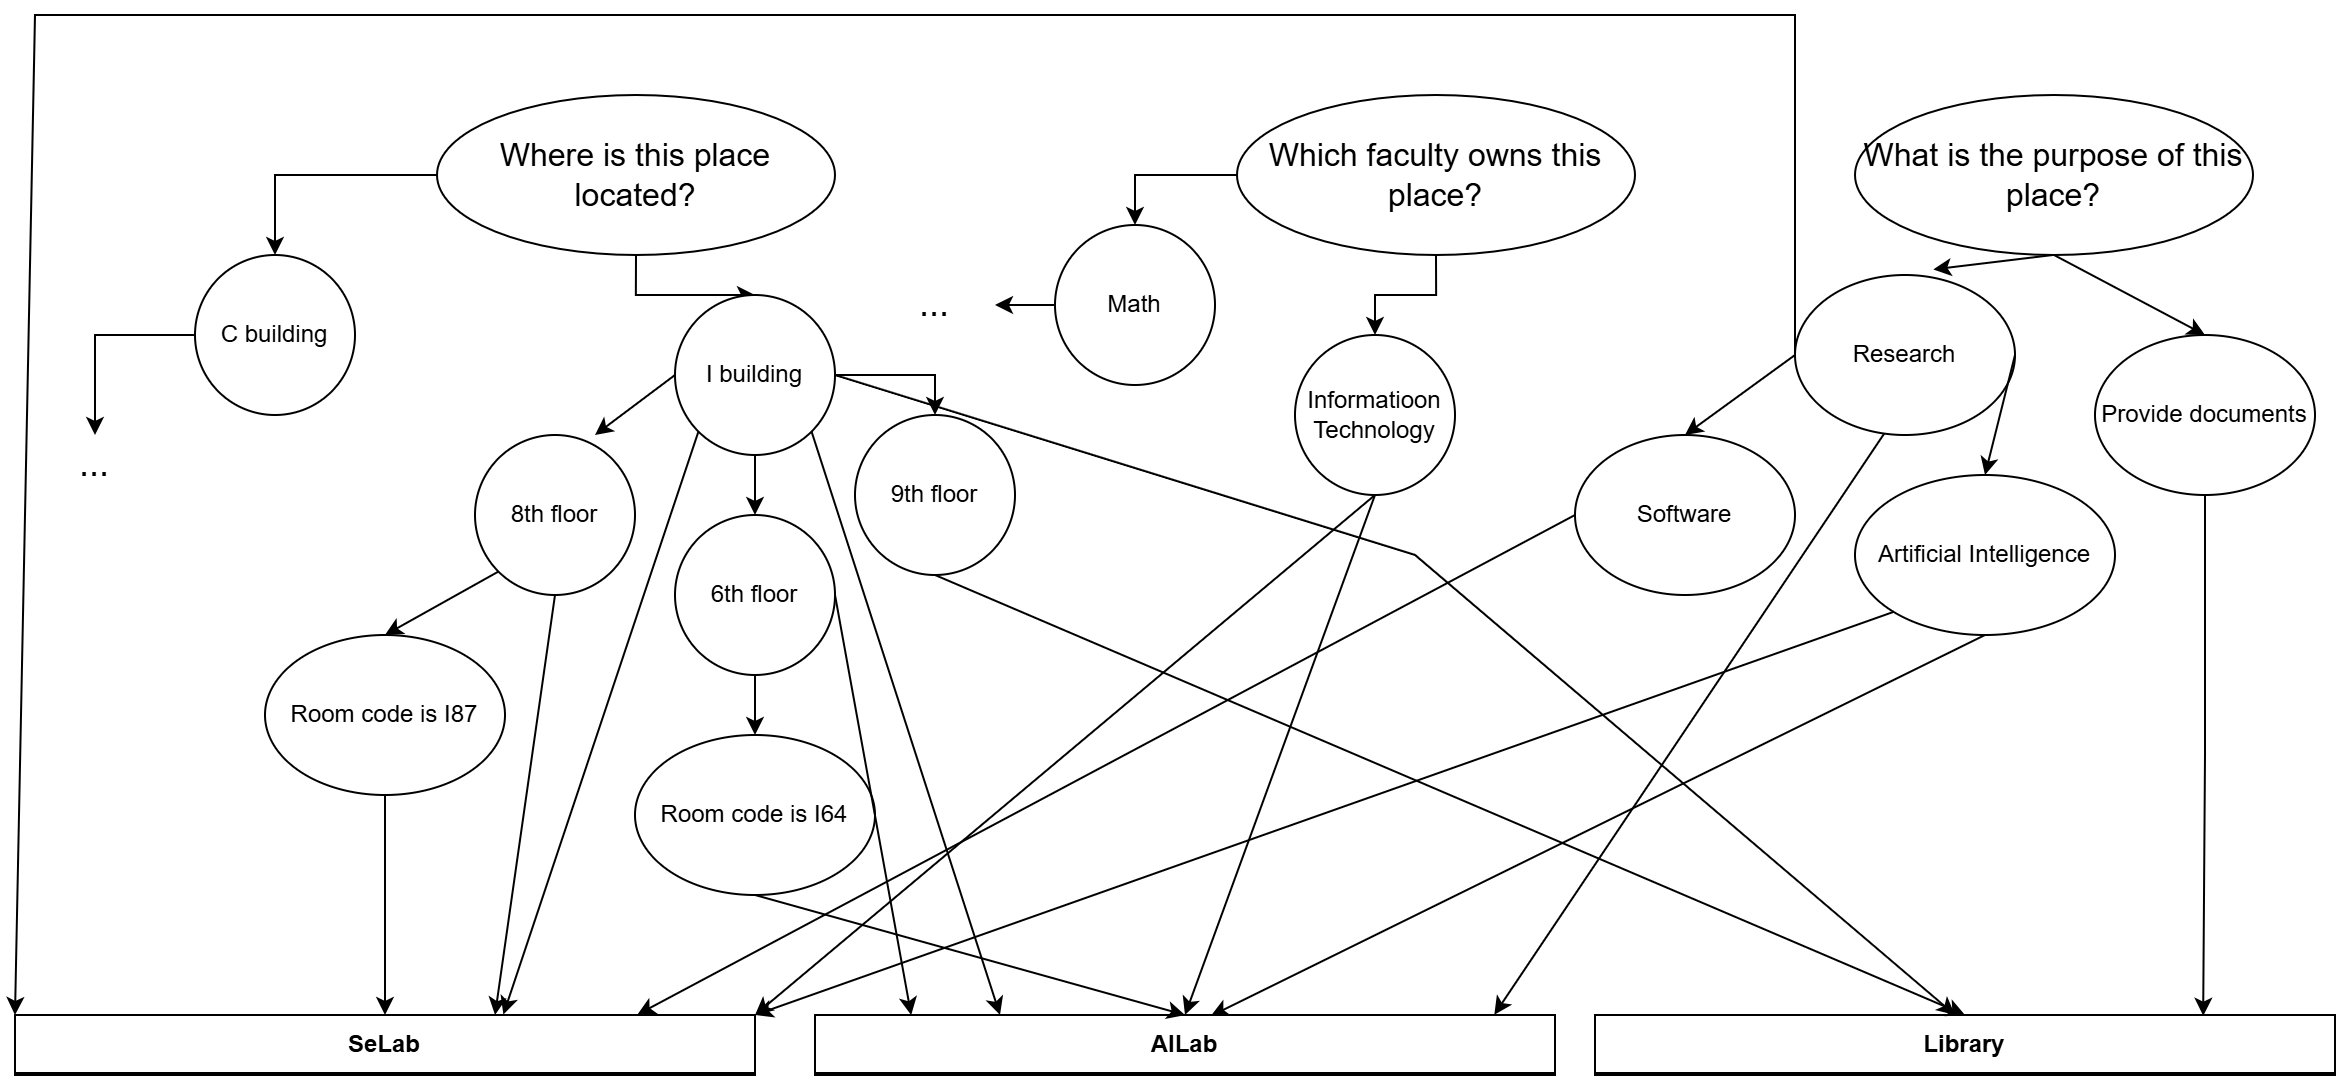
\includegraphics[scale=0.2]{content/resources/images/chap-problems-solutions/data-management-3.png}
  \caption{Hierarchical Data Structure of the three rooms at HCMUS.}
  \label{fig:data-management-3}
\end{figure}

Overall, the hierarchy can be represented as a Directed Acyclic Graph (DAG). We organize places (e.g., SeLab, AILab, Library) according to several attributes. These attributes are grouped under root-level questions, shown at the figure's top. The details are as follows:
\begin{itemize}
\item \textbf{The roots} are the questions pertaining to specific attributes of the places. In other words, each root node corresponds to a fundamental query. These questions do not directly connect to the places; rather, they serve as the entry points for the attribute hierarchy.
\item \textbf{The non-leaf nodes} are the answers for their roots describing the attributes, with the parents containing a generalization of all of their children.
\item \textbf{The leaves} are the actual places themselves (e.g., SeLab, AILab, Library). A leaf node is reached by traversing the path of attributes that fully describe it. The presence of an edge from a non-leaf node to a leaf indicates that the place satisfies the description provided by that node.
\end{itemize}

There is an edge from a non-leaf node to a leaf if the place matches the description in that node. Since a parent contains the generalized description of its children, if there is an edge from a node to a leaf, there must also be an edge from its parent to the leaf, except for the root, as exemplified in Figure~\ref{fig:data-management-4}. With this principle, each attribute can contribute to the finding process at different levels of specificity. For example, if the user asks to find a place with the I87 room, the \texttt{SeLab} can be immediately found (Figure~\ref{fig:data-management-5}). However, suppose the user provides a more vague destination, like finding a room in the I building. In that case, we can still use this information to indicate that the desired destination must be among the three places: \texttt{SeLab}, \texttt{AILab}, or \texttt{Library} (Figure~\ref{fig:data-management-6}). This helps narrow down the search pool of places. Figures~\ref{fig:data-management-7} and~\ref{fig:data-management-8} show the other two common cases.

\begin{figure}[ht]
  \centering
  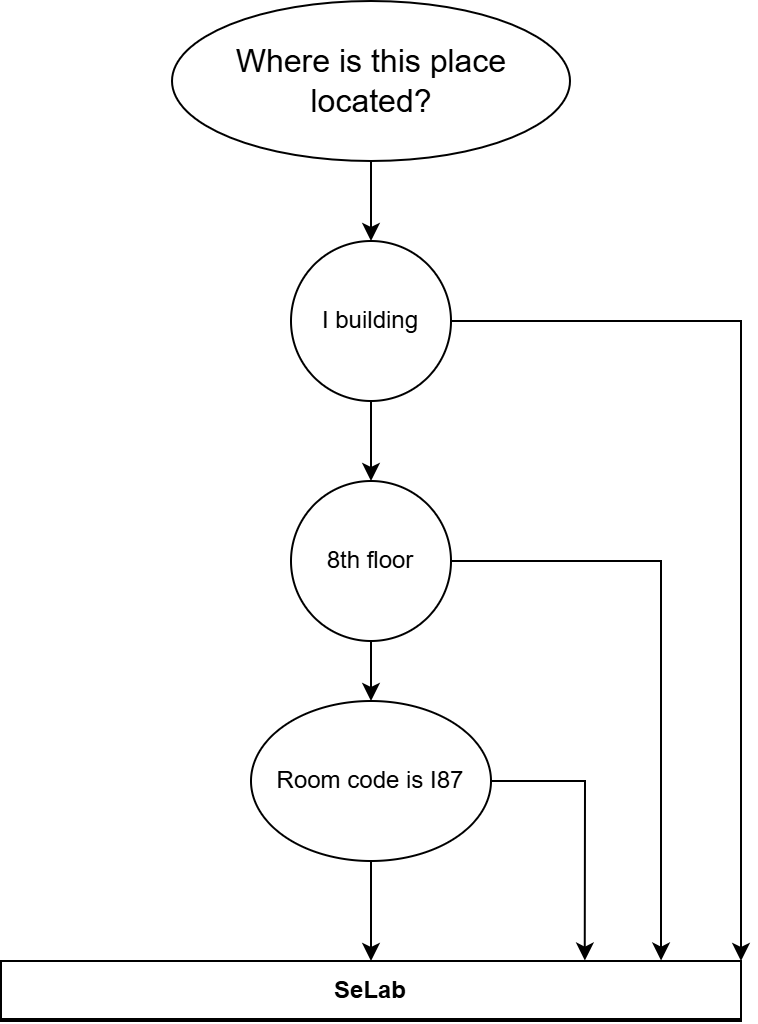
\includegraphics[scale=0.3]{content/resources/images/chap-problems-solutions/data-management-4.png}
  \caption{Leaf's attribute references.}
  \label{fig:data-management-4}
\end{figure}

\begin{figure}[ht]
  \centering
  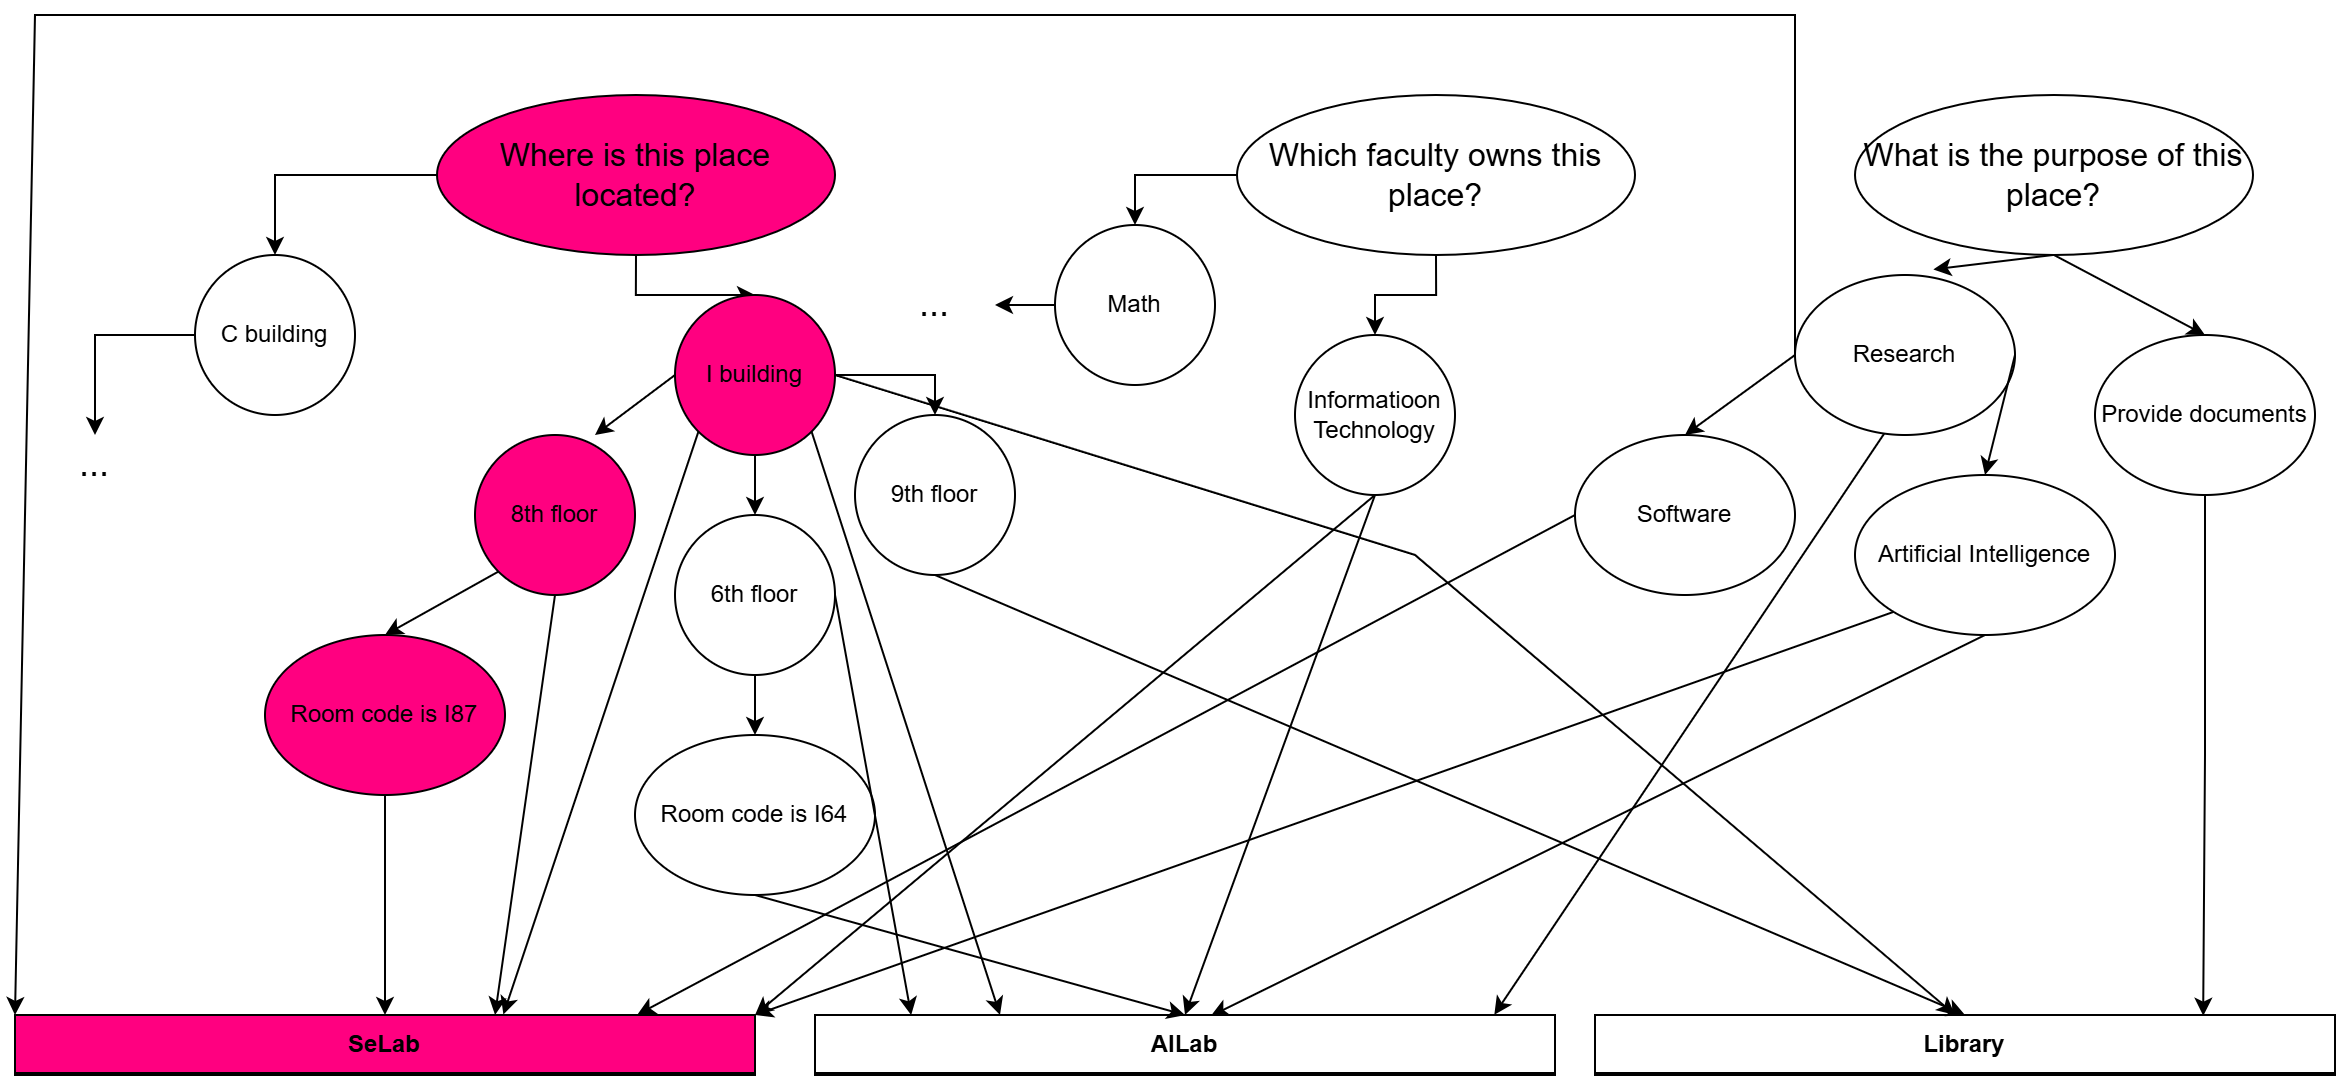
\includegraphics[scale=0.2]{content/resources/images/chap-problems-solutions/data-management-5.png}
  \caption{Find the exact place with detailed information.}
  \label{fig:data-management-5}
\end{figure}

\begin{figure}[ht]
  \centering
  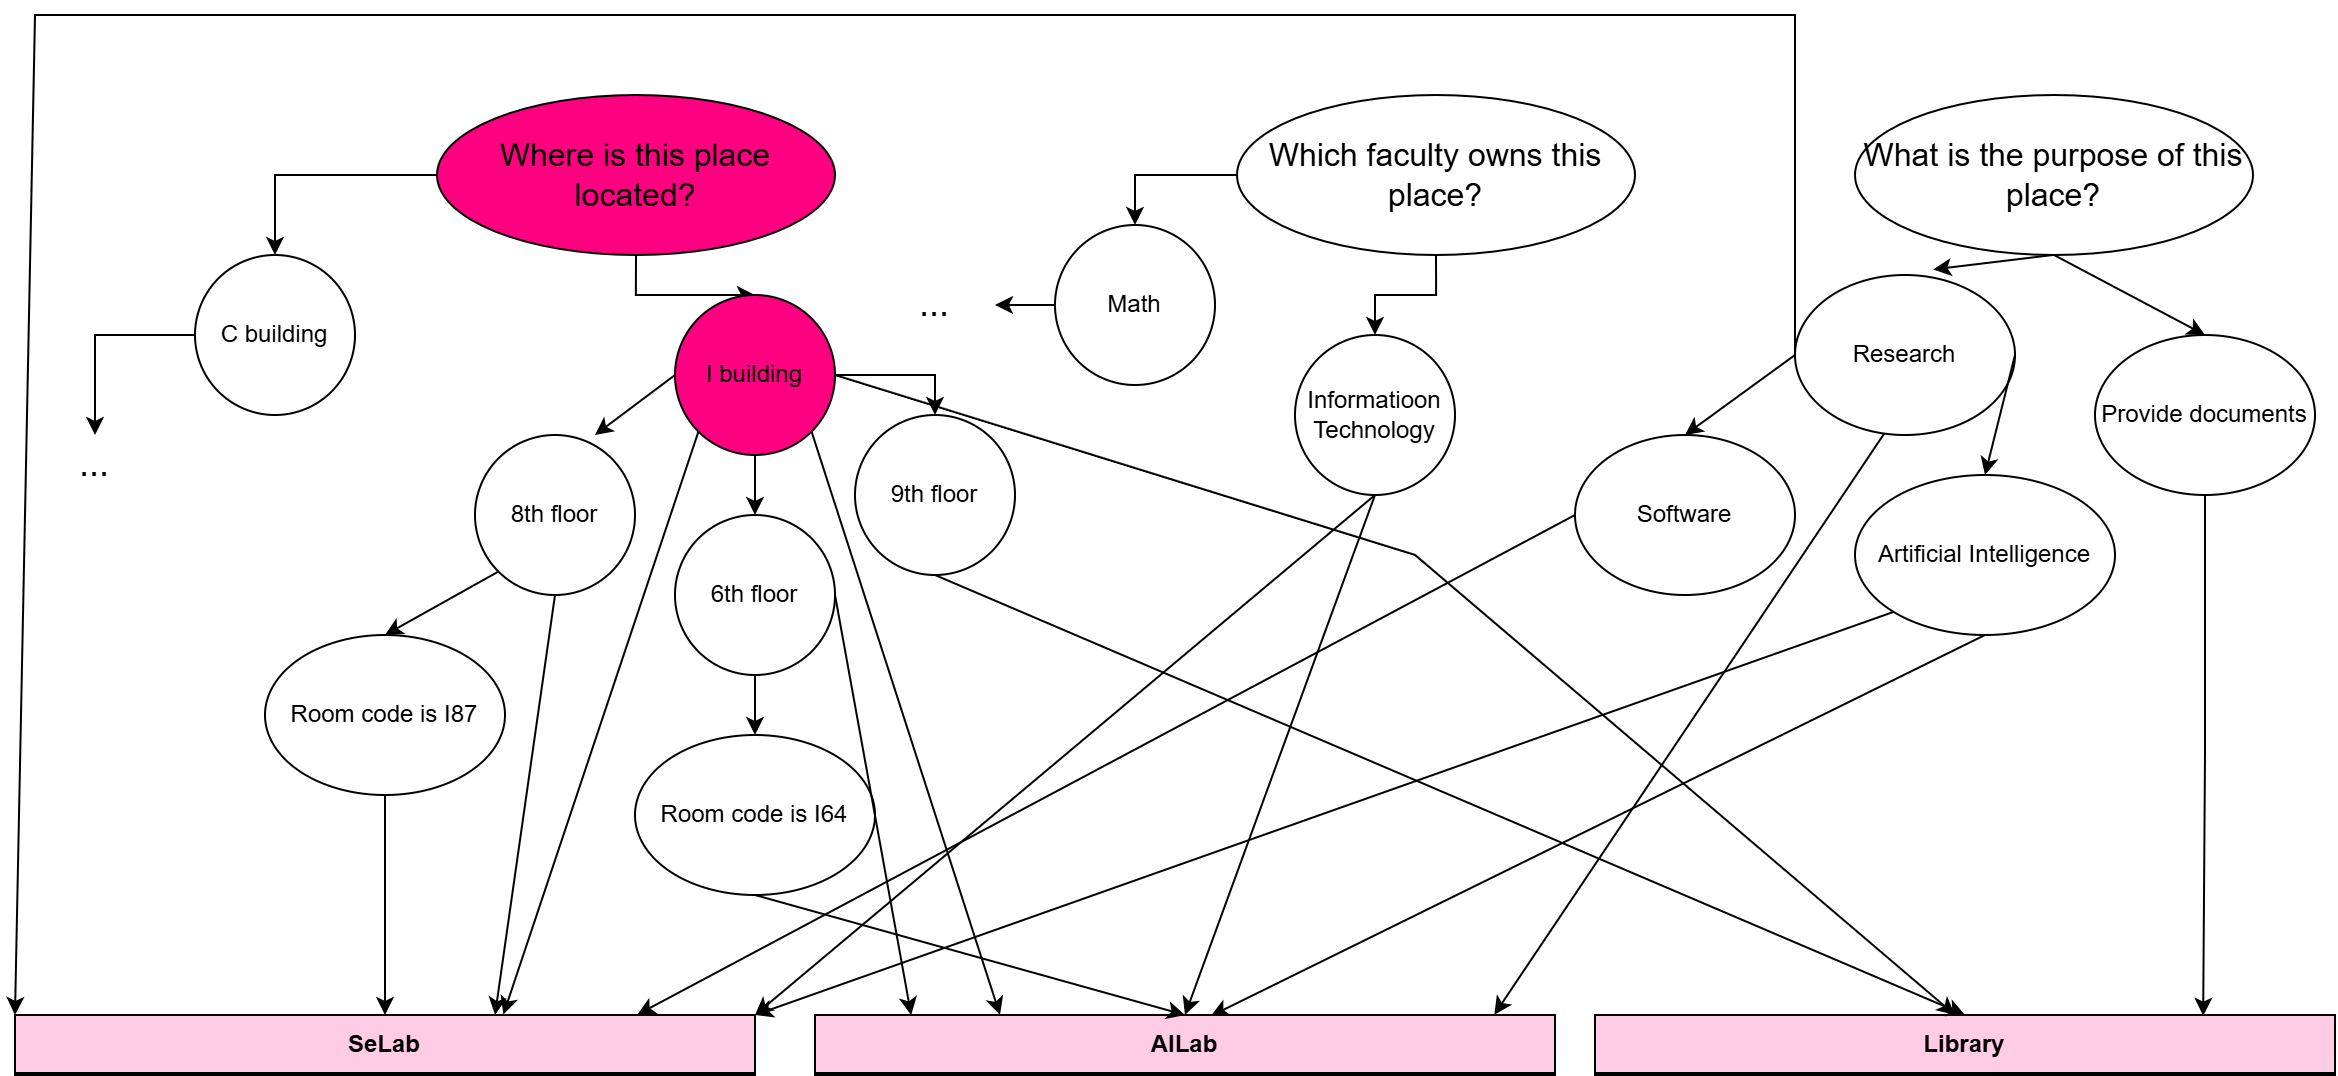
\includegraphics[scale=0.2]{content/resources/images/chap-problems-solutions/data-management-6.png}
  \caption{Narrow down the search range with more generalized information.}
  \label{fig:data-management-6}
\end{figure}

\begin{figure}[ht]
  \centering
  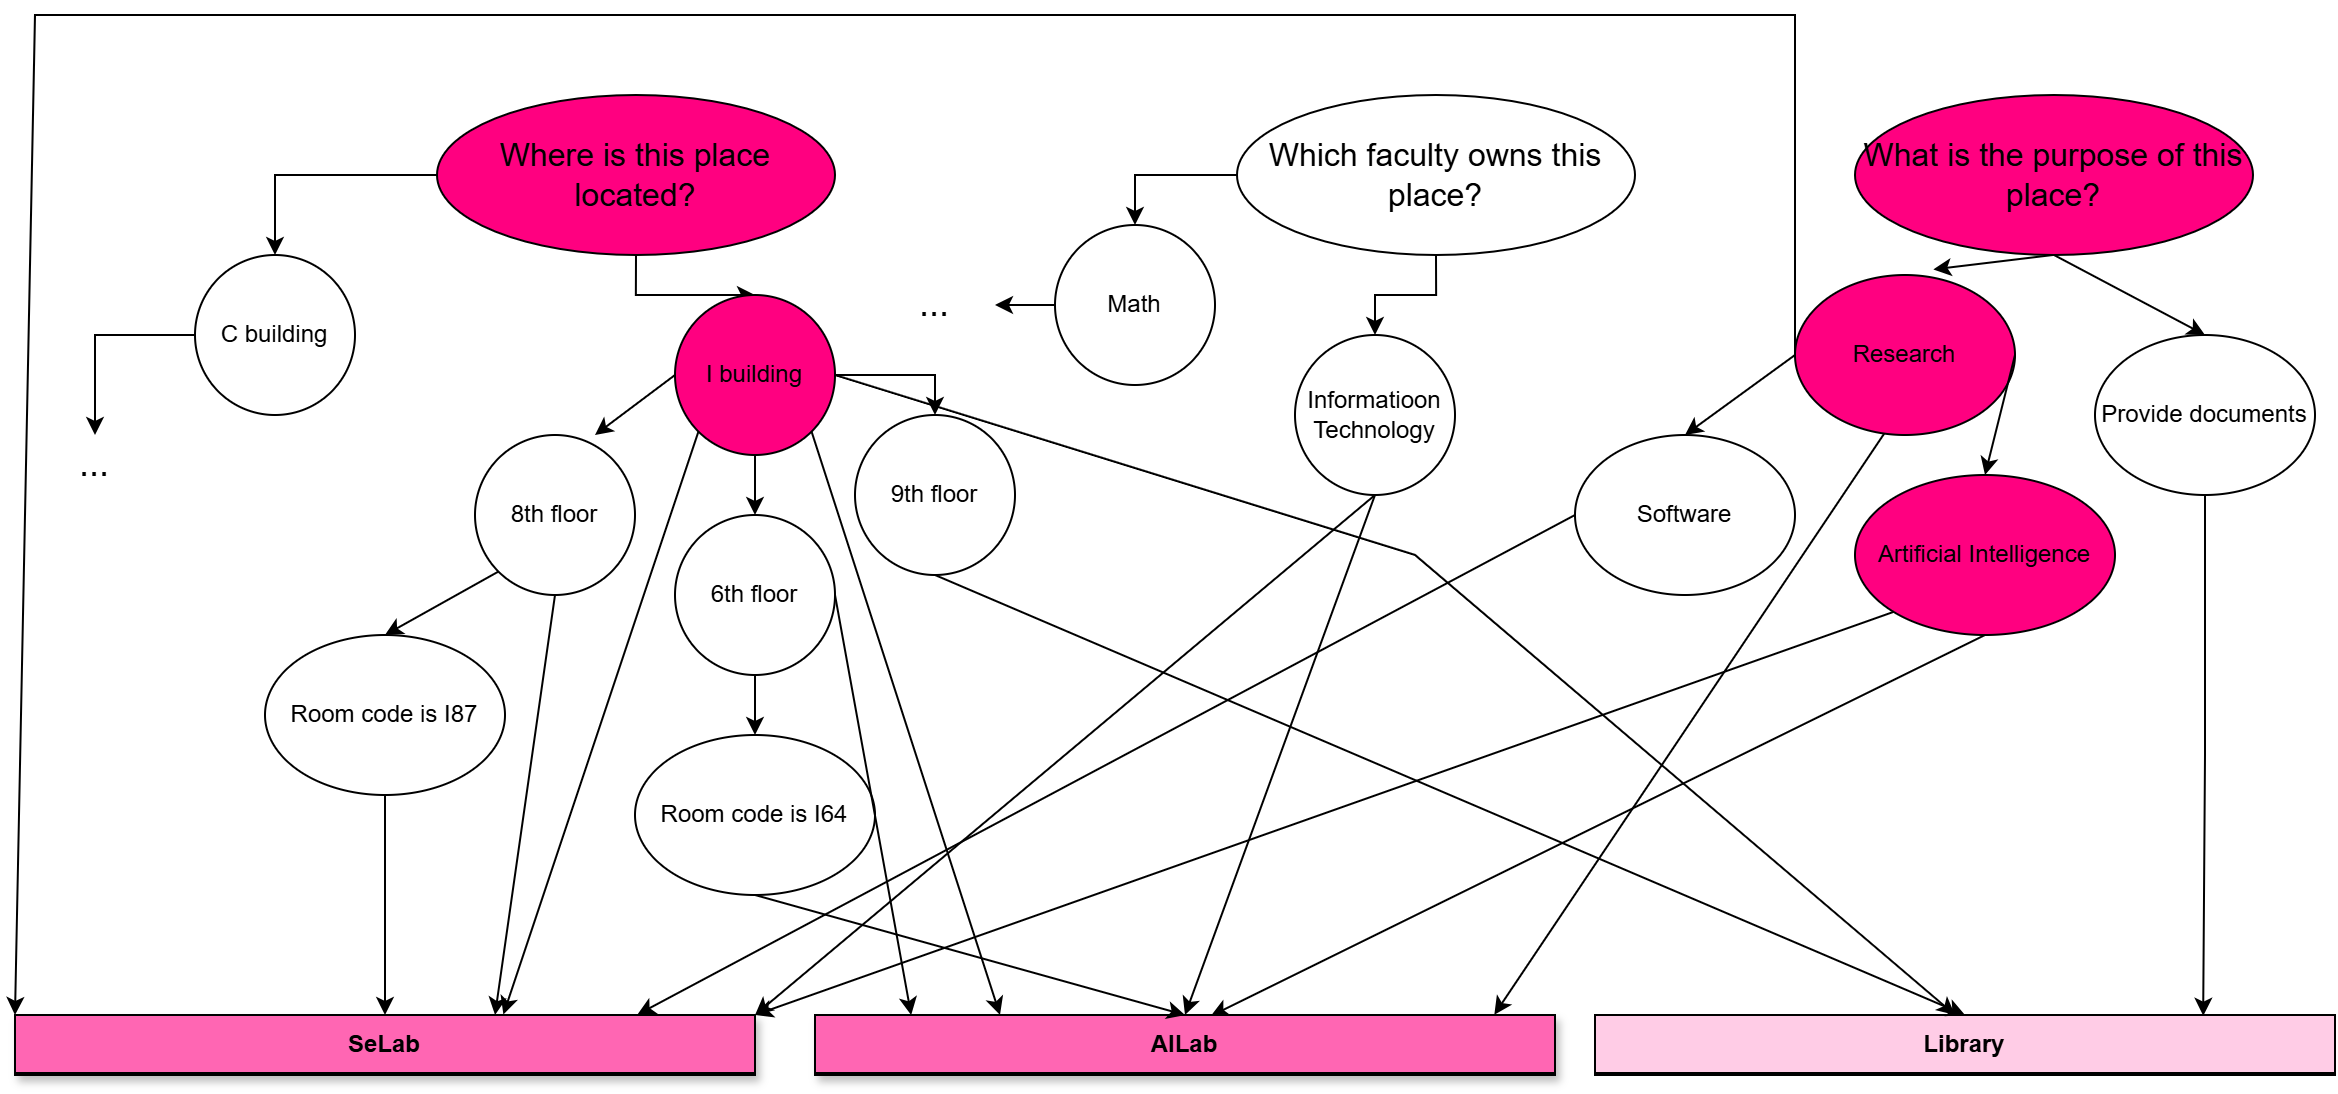
\includegraphics[scale=0.2]{content/resources/images/chap-problems-solutions/data-management-7.png}
  \caption{Narrow down the searching space with \texttt{SeLab} and \texttt{AILab} being the potential candidates.}
  \label{fig:data-management-7}
\end{figure}

\begin{figure}[ht]
  \centering
  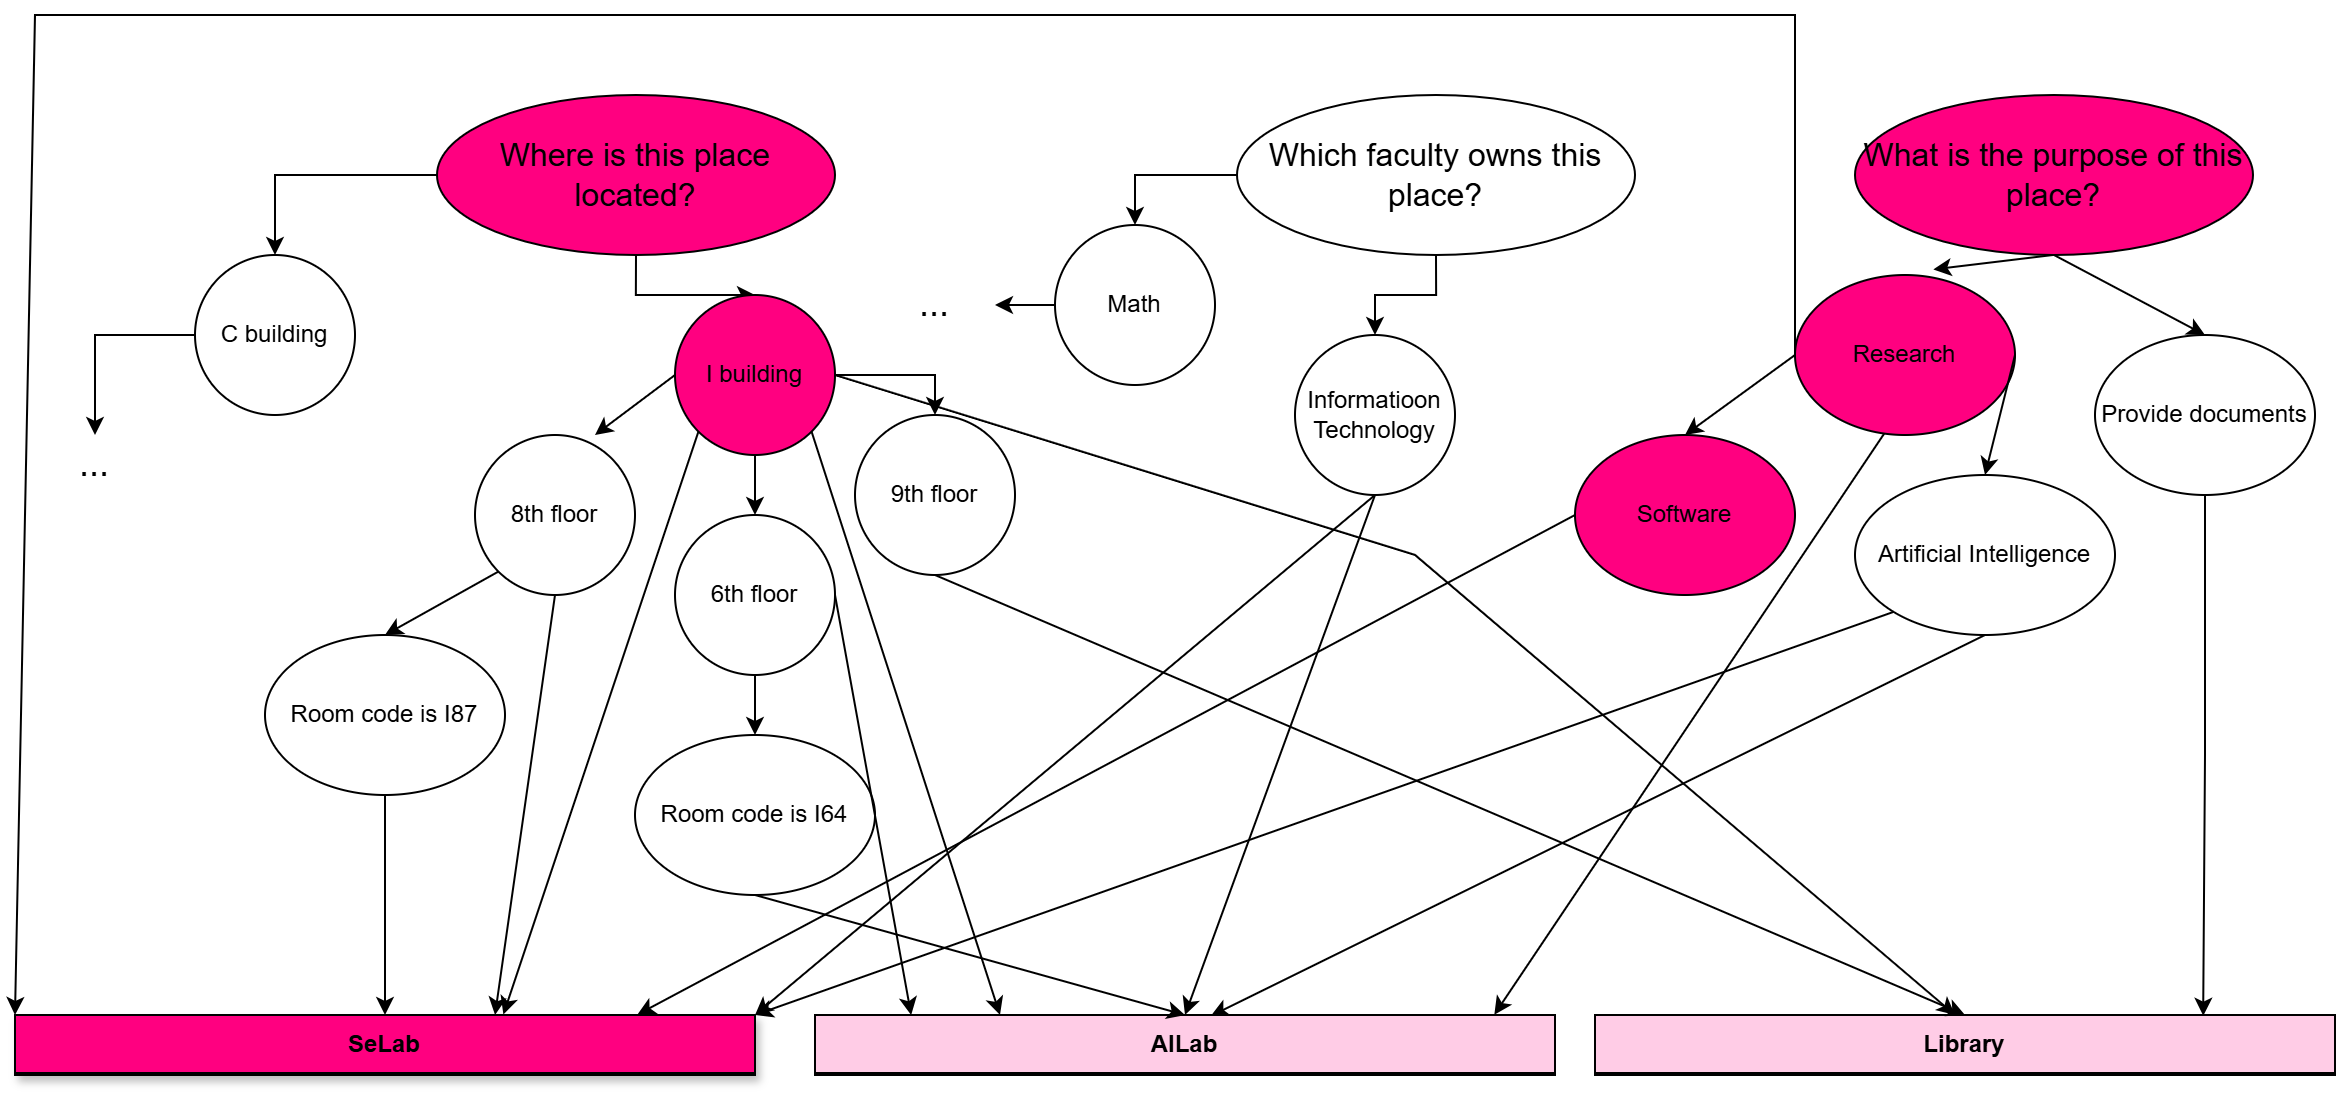
\includegraphics[scale=0.2]{content/resources/images/chap-problems-solutions/data-management-8.png}
  \caption{Searching the exact place with only one most potential candidate being \texttt{SeLab}.}
  \label{fig:data-management-8}
\end{figure}

The hierarchy can be as follows:
\begin{lstlisting}[style=cSharp]
public class HierarchicalDataStructure {
    public const int ROOT = 0;
    public const int SUB_ROOT = 1;
    public const int INTERMEDIATE_NODE = 2;
    public const int LEAF_NODE = 3;
    List<Node> nodes;
}
\end{lstlisting}

A node in the hierarchy can be as follows:

\begin{lstlisting}[style=cSharp]
public class Node {
    public int id;
    public int type;
    public HashSet<int> children;
    public string data;
    public List<String> rules;
}
\end{lstlisting}

The \texttt{id} is the internal id in the hierarchy, which is used for referencing the nodes through a single array \texttt{nodes}. There are four types of nodes, with the \texttt{ROOT} being simply a dummy node for accessing the hierarchy, and the \texttt{SUB\_ROOT}, \texttt{INTERMEDIATE\_NODE}, and \texttt{LEAF\_NODE} corresponding to the roots, non-leaf nodes, and leaves as mentioned above, respectively. The \texttt{children} is the list of links to the lower nodes. The \texttt{data} is:
\begin{itemize}
\item For \texttt{ROOT}: empty, since it is just a dummy node.
\item For \texttt{SUB\_ROOT}: The question that this node represents.
\item For \texttt{INTERMEDIATE\_NODE}: The answer for its \texttt{SUB\_ROOT}, which becomes more specific as one goes downward.
\item For \texttt{LEAF\_NODE}: The information of the place, including its \texttt{id} in the database (as mentioned in Section~\ref{subsubsub:QA-pairs}) for querying the full set of Q\&A pairs if needed. It can also contain some basic information for the place, such as name or position, for immediate usage.
\end{itemize}

The \texttt{rules} is an optional field for the \textt{SUB\_ROOT} only, which is used to define additional rules for each attribute, as discussed in Section~\ref{subsubsubsub:rules}

\subsubsubsubsection*{Query a Place with User's Description}
For a user's description, we also generate the Q\&A pairs. For each pair, we compare the question with the roots to determine if there is a match. If so, we start traversing from that root using the answer in the generated pair to find the most detailed matching attribute. Once we reach the most detailed description possible, we increment the attribute count for all the places referenced. The process is repeated until all pairs are processed, and the place with the highest attribute count will be considered the desired destination. If there are many matching places, we might prompt the user to provide more details about the place, or we might retrieve the complete list of Q\&A pairs for all the found destinations and feed them to the LLM for more detailed matching, as described in Section~\ref{description-matching}. Since the list of places is now much narrower, this operation will be much less costly than previously described.

For now, finding the best matching node is handled through the LLM (specifically ChatGPT's API) to capture the full semantic and contextual meaning best. The nodes are processed by the prompts as follows:
\begin{itemize}
    \item For \texttt{SUB\_ROOT} representing the question, we use the following prompt:
\begin{lstlisting}[style=cSharp]
You are given a pair of text entries: a "Question" and a "Query". Your task is to determine whether the Query provides sufficient information to either directly answer the Question or to allow further classification of potential answers. Follow these rules:
1/ If the Query directly answers the Question, return YES.
2/ If the Query only partially answers the Question but still gives information that can be used to narrow down the possibilities (for example, indicating proximity to a specific room number), return YES.
3/ Otherwise, return NO.
Your output must be exactly one word, either YES or NO, on a single line with no additional text, spaces, or blank lines.
\end{lstlisting}
    \begin{itemize}
        \item Ensure the query accurately matches the question.
        \item Accept the case where the answer might not transparently answer the question but does provide useful information, handling the case mentioned in Section~\ref{no-information-gain}.
        \item Ensure the correct response format.
    \end{itemize}
    
    \item For \texttt{INTERMEDIATE\_NODE} representing an attribute, we use the following prompt:
\begin{lstlisting}[style=cSharp]
You are given a question, a query, and several candidate answers in the format "ID: description". Here, the 'Question' asks for an attribute and the 'Query' is the user’s description of the desired attribute. Following the Query, each line provides a candidate answer where the first candidate is a generalization (i.e., the parent) of all subsequent, more specific answers. Your task is to select the best matching candidate IDs based on the following rules:
1. If the Query is not specific enough and only aligns with the generalization, return only the first candidate's ID.
2. If the Query provides specific information that matches one or more specific candidates, return all matching candidate IDs (each on its own line).
3. If the Query explicitly negates or does not match any candidate when specificity is expected, return an absolutely empty message.
4. If there is an exact match, return only that candidate's ID.
5. If the Query is vague but still permits multiple possibilities, return all candidate IDs that could be valid given the Query, excluding any that are explicitly ruled out.

Your output must contain only the matching candidate IDs (or nothing — an absolutely empty message), with each ID on a separate line and no extra text, spaces, or blank lines.

Examples:
Example 1 (Exact Match):
Question: What is the purpose of this room?
Query: This room is for software engineer research
2: The room purpose is for researching
4: The room purpose is for software engineer research
17: The room purpose is for biology research
Output:
4

Example 2 (Not Specific Enough):
Question: What is the purpose of this room?
Query: This is a laboratory
2: The room purpose is for researching
3: This room is for software engineer research
4: This room is for biology research
Output:
2

Example 3 (Specific but No Match):
Question: What is the purpose of this room?
Query: This room is for math research
2: The room purpose is for researching
3: This room is for software engineer research
4: This room is for biology research
Output:
\end{lstlisting}
    \begin{itemize}
        \item Summarize the context for better contextual handling.
        \item Ensure the query reaches the appropriate level of generalization for the attribute, handling the case mentioned in Section~\ref{not-generalized}.
        \item Correctly utilize other types of information for classifying the nodes, for example, the negation cases, handling the case mentioned in Section~\ref{no-information-gain}.
        \item Exemplify some pivotal cases for accurate handling.
        \item Ensure the correct response format.
    \end{itemize}

\end{itemize}

To confidently ensure the response formats are accurate, all responses will be refined as mentioned in Section~\ref{refine-session}.

For each node, we process it with the following function:

\begin{lstlisting}[style=cSharp]
public async Task TraverseTreeQuery(int id, string query, string sub_root_question = "")
\end{lstlisting}

The details of this function are as follows:
\begin{itemize}
    \item This is a recursive function that is called for each node matching the previous query to traverse further in the hierarchy.
    \item \texttt{id} is the id of the current node being processed.
    \item \texttt{query} is a sentence representing a queried attribute.
    \item \texttt{sub\_root\_question} is the question of the corresponding \texttt{SUB\_ROOT} to capture the context better when matching the query with the answers.
\end{itemize}

When reaching the deepest node (i.e., when it cannot be more specific for the current query), we update the count for places, which are the \texttt{LEAF\_NODE}, as follows:

\begin{lstlisting}[style=cSharp]
foreach (int child in nodes[id].children) {
    if (nodes[child].type == LEAF_NODE) {
        if (matches.ContainsKey(child)) {
            matches[child]++;
        }
        else {
            matches[child] = 1;
        }
    }
}
\end{lstlisting}

Note that a bottleneck in this hierarchy is the response time from the LLM at each node. Although the processed nodes might eventually reference the same leaf nodes, those leaves are also the only shared nodes. Therefore, we consider each node as a separate branch that can be processed concurrently, and thus many requests to the LLM will be sent concurrently, reducing the total response time. Finally, \texttt{ConcurrentDictionary}, a thread-safe hash map in C\#, can handle concurrent leaf node matching. Below is how we use \texttt{Task} for processing the branches concurrently:

\begin{lstlisting}[style=cSharp]
List<Task> tasks = new List<Task>();

// Traverse the tree
foreach (int child in nodes[root].children) {
    foreach (string query in queries) {
        tasks.Add(TraverseTreeQuery(child, query));
    }
}
await Task.WhenAll(tasks);
\end{lstlisting}

Below is an example of processing a query (Figure~\ref{fig:data-management-8}). Consider the query:

\begin{lstlisting}[style=cSharp]
Find me the software lab in I building. 
\end{lstlisting}

The generated pairs are:

\begin{lstlisting}[style=cSharp]
What is the purpose of this room?
This room is a software laboratory.
What is the building of this room?
This room is in the I building.
\end{lstlisting}

Comparing each pair of questions from \texttt{SUB\_ROOT} nodes and the generated ones, we have two matches: \texttt{(What is the location of this lab?, Where is this place located?)} and \texttt{(What is the purpose of this room?, What is the purpose of this room?)}.

For the first question, the LLM then responds with the \texttt{I building} node as the best match. After that, when processing the \texttt{I building} node, the LLM responds that the only match is the \texttt{I building} node, which is the current node itself. This means that we have reached the deepest possible level of specification for this question, given the query; therefore, all of its children, including all three rooms, are marked as matches.

For the second question, the LLM then responds with the \texttt{Research} node as the best match, and then \texttt{Software} as the best match. Since this node has no other \texttt{INTERMEDIATE\_NODE} children, we have reached the deepest level of specification. Therefore, its only child, \texttt{SeLab}, is marked.

Finally, since the only leaf with the highest attribute count, this is the desired destination since \texttt{SeLab} is the only leaf with the highest attribute count.

\subsubsubsubsection*{Add a New Place to the Hierarchy}
First, a new \texttt{LEAF\_NODE} representing the new place is created. Similar to the querying process, using the metadata of the place (i.e., the set of Q\&A pairs), we traverse the existing hierarchy to find any matching attributes and reference them to the new node. When there are no matches, we create a new node with the following prompt:

\begin{lstlisting}[style=cSharp]
I want to build a hierarchy for a room/place in the campus.
Given the following attribute description that is to answer the below question.
Please consider the following two cases:
    1. If the description can be generalized, return the generalized description.
    2. Otherwise, return the description itself.
For example, if the question is ""What is the purpose of this room?"", and the description is ""The room is for computer science research"".
In this case, return ""The room is for research purposes"", since it is more general.
Another example, if the question is ""What is the room number?"", and the description is ""The room number is I87"".
In this case, return ""The room number is I87"", since it cannot be generalized.
Just return description, NO OTHER WORDS OR CHARACTERS.
\end{lstlisting}

This prompt:
\begin{itemize}
    \item Summarizes the context for better contextual handling.
    \item Generates the descriptive data for this node for the new place. If possible, it also attempts to create a generalized description for handling the case mentioned in Section~\ref{not-generalized}.
    \item Correctly utilizes other types of information for classifying the nodes, for example, the negation cases, handling the case mentioned in Section~\ref{no-information-gain}.
    \item Exemplifies some pivotal cases for accurate handling.
    \item Ensures the correct response format.
\end{itemize}

For example, consider adding a place with the following Q\&A pairs metadata:

\begin{lstlisting}[style=cSharp]
What is the purpose of this place?
The purpose of this place is for researching microbiology.
Which faculty does this place belong to?
This place belongs to the Biology Faculty.
\end{lstlisting}

The hierarchy is updated as in Figure~\ref{fig:data-management-9}. In this figure, the pink nodes are the nodes that matched the new place's attributes, while the blue ones are the newly created nodes. As we can see, three common cases are being exemplified here:
\begin{itemize}
\item The questions and the \texttt{Research} node are reused since those match the new attributes.
\item The \texttt{Biology} node (the one under the \texttt{Which faculty owns this place?} node) is created as described in the metadata.
\item The \texttt{Biology} node (the one under the \texttt{Research} node), although not explicitly described in the metadata, is created as a generalization of the \texttt{Microbiology} attribute. This node guarantees the structure of the hierarchy.
\end{itemize}

Using this method in combination with the Q\&A pairs generation mentioned in Section~\ref{subsubsub:QA-pairs}, the entire process of adding a new place with a raw description to the data structure can be fully automated.

\begin{figure}[ht]
  \centering
  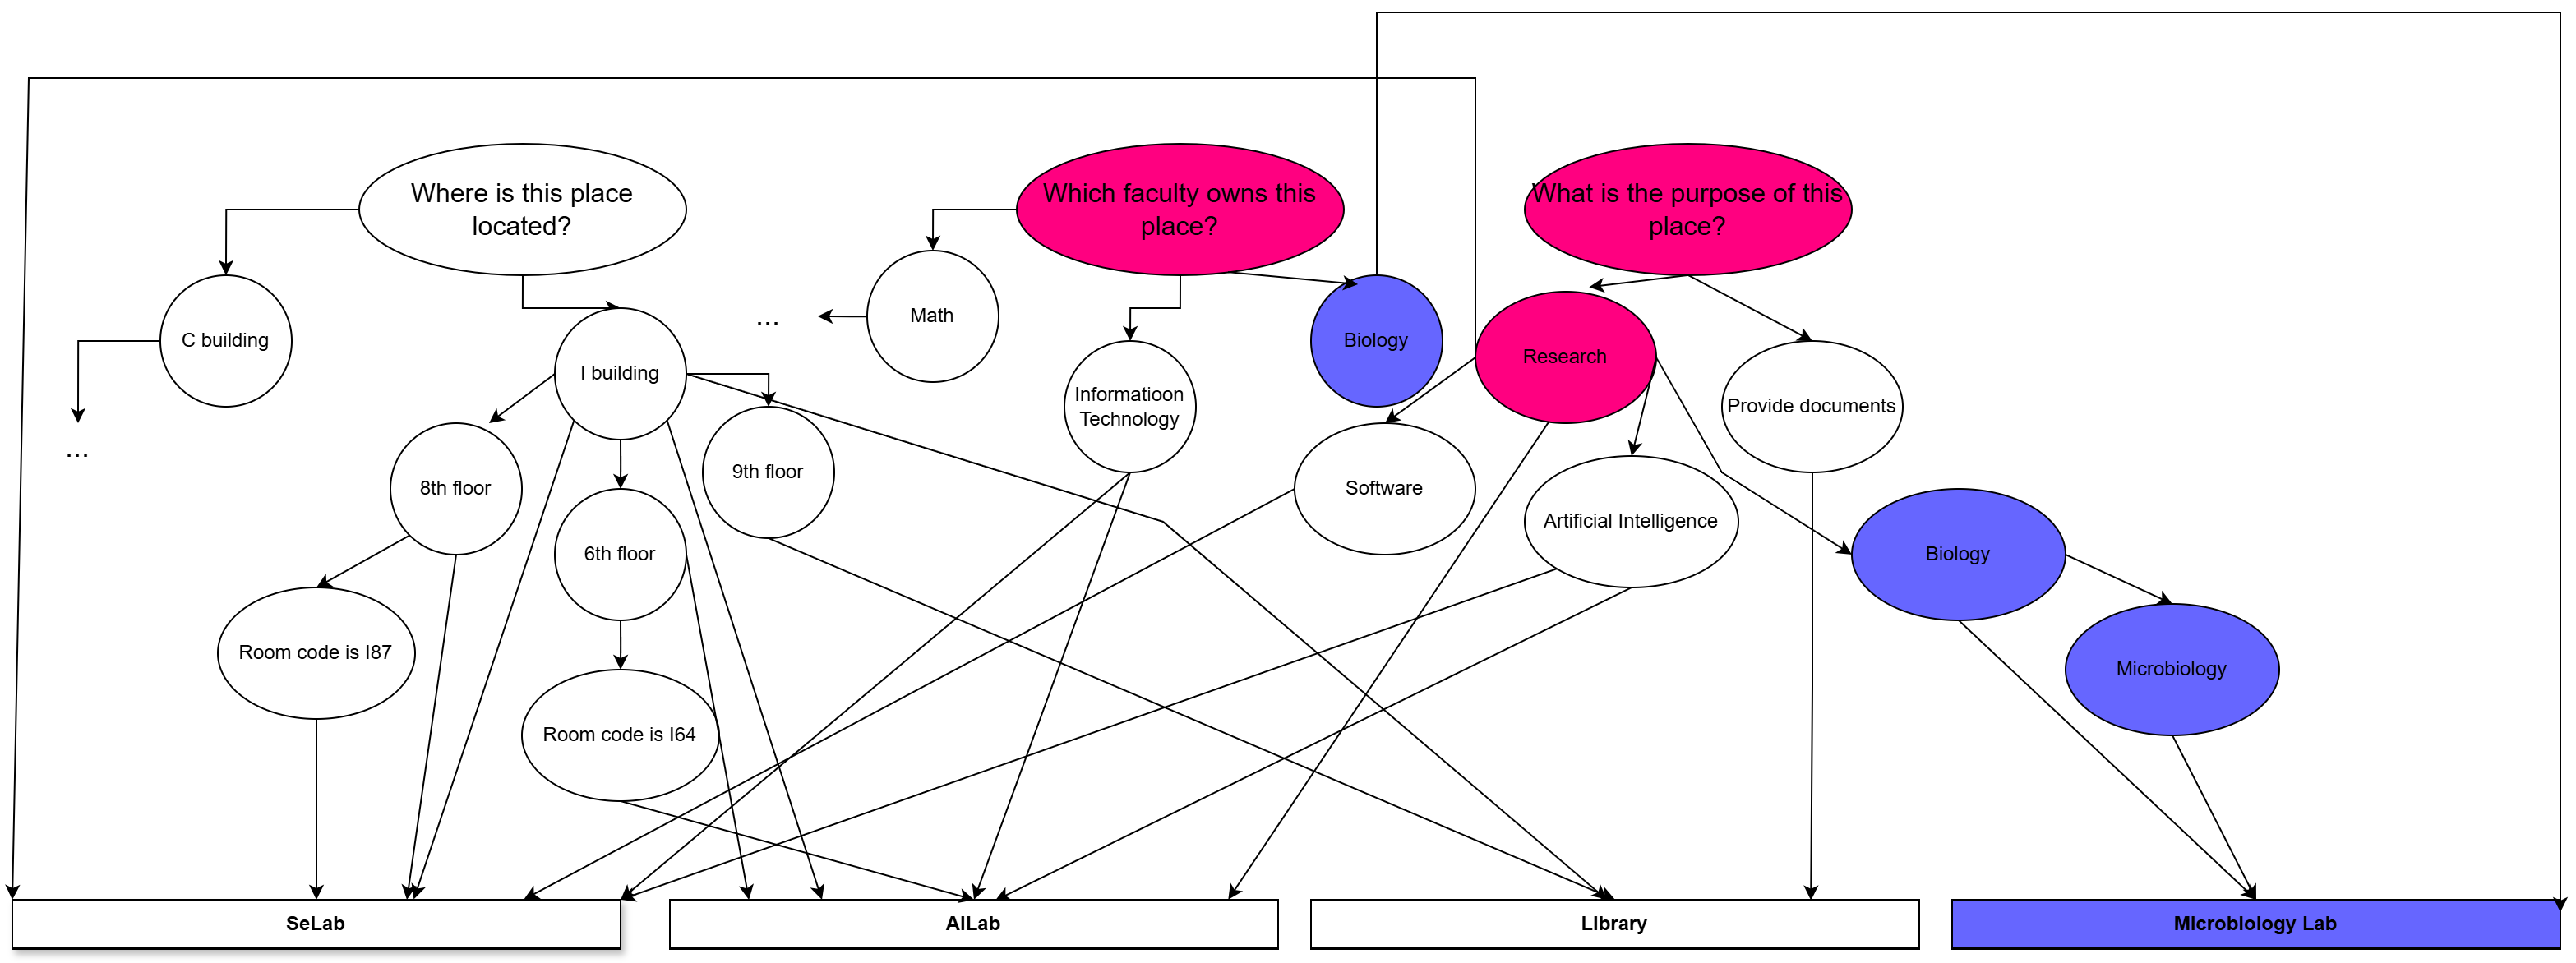
\includegraphics[scale=0.15]{content/resources/images/chap-problems-solutions/data-management-9.png}
  \caption{The hierarchy being updated with \texttt{Microbiology Lab}.}
  \label{fig:data-management-9}
\end{figure}

\subsubsubsubsection*{Add a new rule}\label{subsubsubsub:rules}
With each attribute on a different \texttt{SUB\_ROOT}, users can manually define new rules that can be considered when querying. The process of adding a new rule can also be done automatically, as follows:
\begin{lstlisting}[style=cSharp]
public async Task AddRule(string rule) {
    OpenAI openAI = new OpenAI();
    Helper helper = new Helper();
    foreach (int sub_root in nodes[root].children) {
        string response = await openAI.OpenAIGetAnswer("\nRule: " + rule + "\nQuestion: " + nodes[sub_root].data, 
@"Please answer if the following rule serves as extra information for defining the structure of the answer for the following question.
Return exactly 'YES' if the query answer the question, 'NO' otherwise.
NO OTHER WORDS
");
        response = helper.refineResponse(response);
        if (response.Contains("YES")) {
            nodes[sub_root].rules.Add(rule);
        }
    }
}
\end{lstlisting}

The users only need to define a new rule, the rule is then matched to the appropriate \texttt{SUB\_ROOT}.

\begin{figure}[ht]
  \centering
  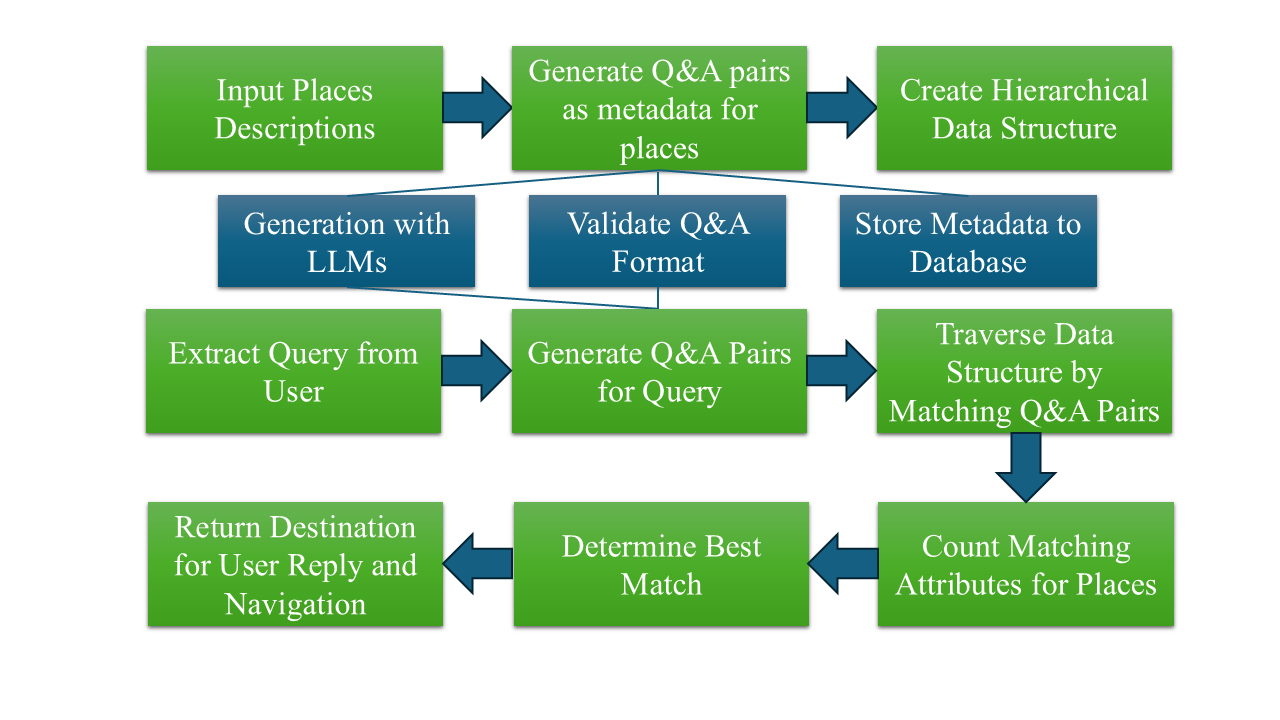
\includegraphics[scale=0.5]{content/resources/images/chap-problems-solutions/data-management-0.png}
  \caption{LLM-Driven Hierarchical Database: Construction and Query Processing Workflow.}
  \label{fig:data-management-0}
\end{figure}
